\documentclass[tikz,border=12pt]{standalone}
\usepackage[T1]{fontenc}
\usepackage{lmodern}
\usetikzlibrary{arrows.meta,calc,fit,backgrounds,positioning}

% Opção A: faixa O-QUÊ em cima, faixa COMO embaixo, pares alinhados
% na mesma coluna, seta reta descendo. Layout bem horizontal (1 linha x 6).

\definecolor{ink}{HTML}{25344A}
\definecolor{quebg}{HTML}{EEF1F7}
\definecolor{queborder}{HTML}{27344A}
\definecolor{comobg}{HTML}{E9F7EE}
\definecolor{comoborder}{HTML}{1F6B3A}

\tikzset{
  box/.style={rectangle, draw=ink, fill=white, rounded corners=2pt,
              line width=0.8pt, align=center, text width=2.6cm,
              minimum height=1.9cm, inner sep=5pt, font=\ttfamily\small},
  conn/.style={-{Latex[length=2.2mm]}, draw=black, line width=0.9pt}
}

\begin{document}
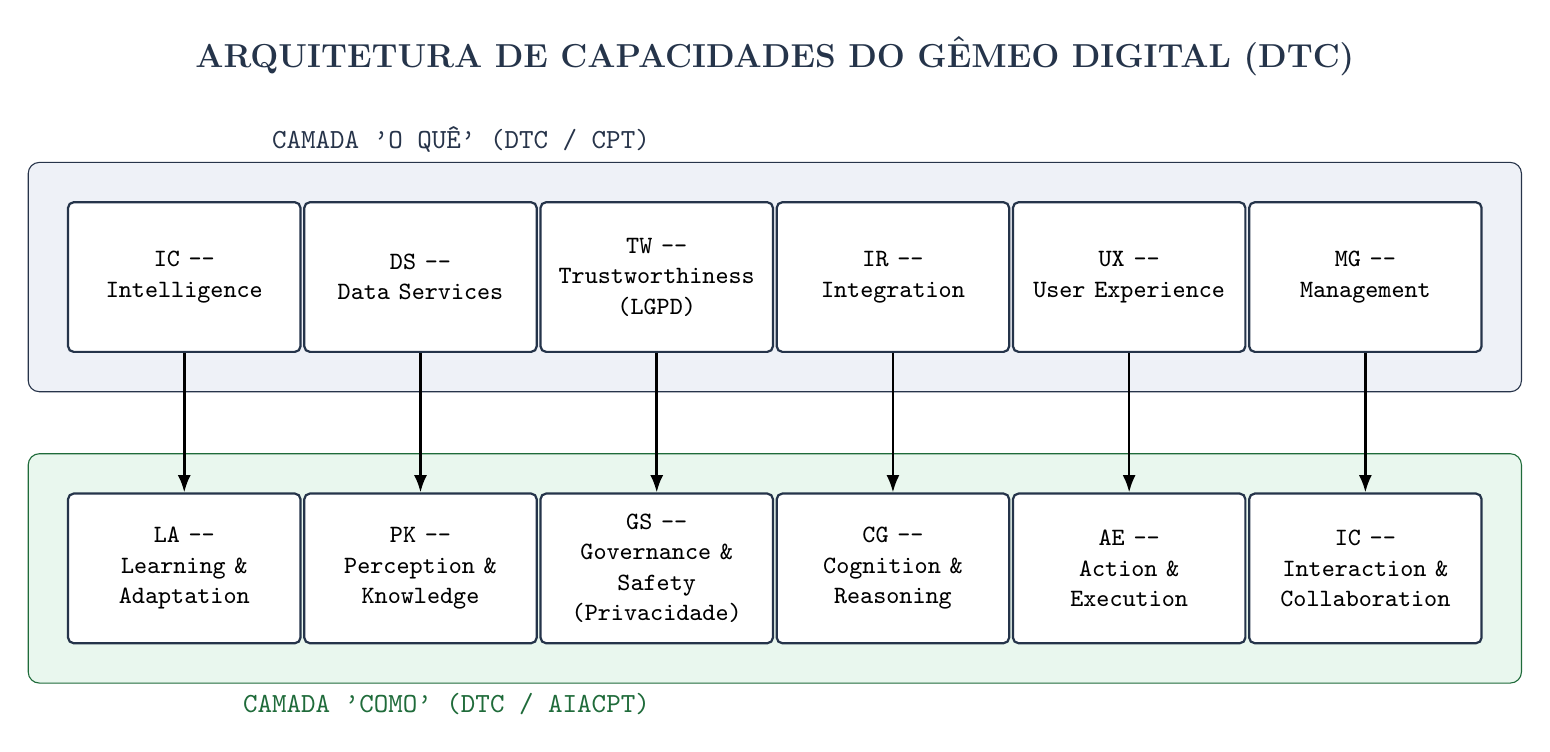
\begin{tikzpicture}[font=\ttfamily]

  \node[font=\bfseries\large, text=ink] at (7.5,7.1)
    {ARQUITETURA DE CAPACIDADES DO GÊMEO DIGITAL (DTC)};

  % ---- Faixa "O QUÊ" (CPT): linha única, 6 colunas ----
  \node[box] (q1) at (0,4.3)  {IC --\\ Intelligence};
  \node[box] (q2) at (3.0,4.3){DS --\\ Data Services};
  \node[box] (q3) at (6.0,4.3){TW --\\ Trustworthiness\\ (LGPD)};
  \node[box] (q4) at (9.0,4.3){IR --\\ Integration};
  \node[box] (q5) at (12.0,4.3){UX --\\ User Experience};
  \node[box] (q6) at (15.0,4.3){MG --\\ Management};

  % ---- Faixa "COMO" (AIACPT): linha única, alinhada em x com O QUÊ ----
  \node[box] (c1) at (0,0.6)  {LA --\\ Learning \&\\ Adaptation};
  \node[box] (c2) at (3.0,0.6){PK --\\ Perception \&\\ Knowledge};
  \node[box] (c3) at (6.0,0.6){GS --\\ Governance \&\\ Safety\\ (Privacidade)};
  \node[box] (c4) at (9.0,0.6){CG --\\ Cognition \&\\ Reasoning};
  \node[box] (c5) at (12.0,0.6){AE --\\ Action \&\\ Execution};
  \node[box] (c6) at (15.0,0.6){IC --\\ Interaction \&\\ Collaboration};

  % ---- faixas de fundo ----
  \begin{scope}[on background layer]
    \node[fill=quebg, draw=queborder, rounded corners=4pt,
          fit=(q1)(q2)(q3)(q4)(q5)(q6), inner sep=14pt,
          label={[font=\ttfamily\bfseries, text=queborder]above left:
                 CAMADA 'O QUÊ' (DTC / CPT)}] {};
    \node[fill=comobg, draw=comoborder, rounded corners=4pt,
          fit=(c1)(c2)(c3)(c4)(c5)(c6), inner sep=14pt,
          label={[font=\ttfamily\bfseries, text=comoborder]below left:
                 CAMADA 'COMO' (DTC / AIACPT)}] {};
  \end{scope}

  % ---- setas: par a par, reto para baixo ----
  \foreach \i in {1,...,6}
    \draw[conn] (q\i.south) -- (c\i.north);

\end{tikzpicture}
\end{document}